%%% In this section, you will describe all of the various artifacts that you will generate and maintain during the project life cycle. Describe the purpose of each item below, how the content will be generated, where it will be stored, how often it will be updated, etc. Replace the default text for each section with your own description. Reword this paragraph as appropriate.

\subsection{Major Documentation Deliverables}
These deliverables are major grade components of the course. Completing these documents should generally be the sprint goal during the applicable sprint period. Refer to current and previous course syllabi and schedules to estimate the due dates of these items. Remove this explanatory paragraph from your draft, but leave the heading.

\subsubsection{Project Charter}
Describe how this document will be maintained and updated (how often, under what circumstances, etc.). When will the initial version be delivered? When will the final version be delivered?

\subsubsection{System Requirements Specification}
Describe how this document will be maintained and updated (how often, under what circumstances, etc.). When will the initial version be delivered? When will the final version be delivered?

\subsubsection{Architectural Design Specification}
Describe how this document will be maintained and updated (how often, under what circumstances, etc.). When will the initial version be delivered? When will the final version be delivered?

\subsubsection{Detailed Design Specification}
Describe how this document will be maintained and updated (how often, under what circumstances, etc.). When will the initial version be delivered? When will the final version be delivered?

\subsection{Recurring Sprint Items}
The following items will be documented and maintained during each individual sprint. As above, remove this paragraph from your draft, but leave the heading.

\subsubsection{Product Backlog}
How will items be added to the product backlog from the SRS? How will these items be prioritized? Who makes the decision (product owner, group vote, etc.)? What software will be used to maintain and share the product backlog with team members and stakeholders?

\subsubsection{Sprint Planning}
How will each sprint plan be planned? How many sprints will there be (you need to look at the schedules for this course and previous Senior Design II courses during the appropriate semesters to figure this out).

\subsubsection{Sprint Goal}
Who decides the sprint goal? How will you involve your customer in this process?

\subsubsection{Sprint Backlog}
Who decides which product backlog items make their way into the sprint backlog? How will the backlog be maintained (collaboration software, a "scrum board", etc.)?

\subsubsection{Task Breakdown}
How will individual tasks be assigned from the sprint backlog? Will it be up to each team member to voluntarily claim a task, or will it come from the product owner? How will time spent on tasks be documented?

\subsubsection{Sprint Burn Down Charts}
Who will be responsible for generating the burn down charts for each sprint? How will they be able to access the total amount of effort expended by each individual team member? What format will the burn down chart use (include an example burn down chart below).

\begin{figure}[h!]
    \centering
    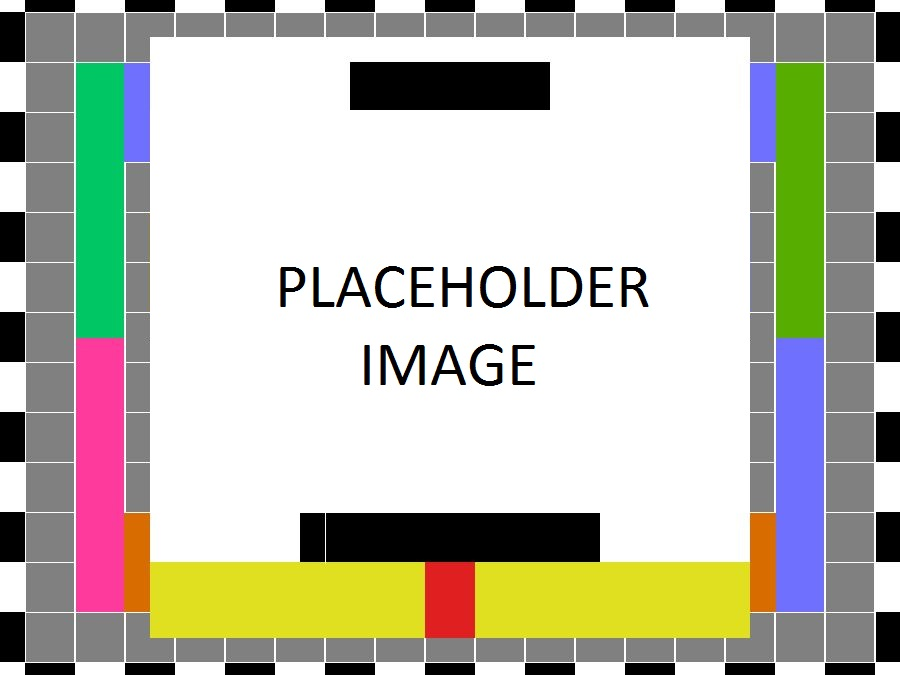
\includegraphics[width=0.5\textwidth]{images/test_image}
    \caption{Example sprint burn down chart}
\end{figure}

\subsubsection{Sprint Retrospective}
How will the sprint retrospective be handled as a team? When will this discussion happen after each sprint? What will be documented as a group and as individuals, and when will it be due?

\subsubsection{Individual Status Reports}
What sort of status will be reported by each individual member, and how often will it be reported? What key items will be contained in the report?

\subsubsection{Engineering Notebooks}
How often will the engineering notebook be updated, at a minimum, by each team member? What is the minimum amount of pages that will be completed for each interval, and how long will that interval be? How will the team keep each member accountable? Who will sign of as a "witness" for each ENB page?

\subsection{Closeout Materials}
The following materials, in addition to major documentation deliverables, will be provided to the customer upon project closeout. Remove this paragraph from your draft, but leave the heading.

\subsubsection{System Prototype}
What will be included in the final system prototype? How and when will this be demonstrated? Will there be a Prototype Acceptance Test (PAT) with your customer? Will anything be demonstrated off-site? If so, will there be a Field Acceptance Test (FAT)?

\subsubsection{Project Poster}
What will be included on the poster, what will be the final dimensions, and when will it be delivered?

\subsubsection{Web Page}
What will be included on the project web page? Will it be accessible to the public? When will this be delivered? Will it be updated throughout the project, or just provided at closeout (at a minimum, you need to provide a simple web page at the end).

\subsubsection{Demo Video}
What will be shown in the demo video(s)? Will you include a B-reel footage for future video cuts? Approximately how long will the video(s) be, and what topics will be covered?

\subsubsection{Source Code}
How will your source code be maintained? What version control system will you adopt? Will source code be provided to the customer, or binaries only? If source code is provided, how will it be turned over to the customer? Will the project be open sourced to the general public? If so, what are the license terms (GNU, GPL, MIT, etc.). Where will the license terms be listed (in each source file, in a single readme file, etc.).

\subsubsection{Source Code Documentation}
What documentation standards will be employed? Will you use tools to generate the documentation (Doxygen, Javadocs, etc.). In what format will the final documentation be provided (PDF, browsable HTML, etc.)?

\subsubsection{Hardware Schematics}
Will you be creating printed circuit boards (PCBs) or wiring components together? If so, list each applicable schematic and what sort of data it will contain (PCB layout, wiring diagram, etc.). If your project is purely software, omit this section.

\subsubsection{CAD files}
Will the project involve any mechanical design, such as 3D printed or laser-cut parts? If so, what software will you use to generate the files and what file formats will you provide in your closeout materials (STL, STEP, OBJ, etc.). If your project is purely software, omit this section.

\subsubsection{Installation Scripts}
How will the customer deploy software to new installations? Will you provide installation scripts, install programs, or any other tools to improve the process? Will there be multiple scripts provided (perhaps separate scripts for the graphical front end and back end server software)? 

\subsubsection{User Manual}
Will you customer need a printed or digital user manual? Will they need a setup video? Decide now what will be provided and discuss.
